\chapter{Multivariate Distributions}

\section{Distributions of Two Random Variables}

\begin{definition}{}{}
    Given a random experiment with a sample space $\mathcal{C}$,
    consider two random variables $X_1$ and $X_2$ which assign to each element $c$
    of $\mathcal{C}$ one and only one ordered pair of numbers $(X_1,X_2)$ is a random vector.
    The space of $(X_1,X_2)$ is the set of ordered pairs $\mathcal{D}=\{(x_1,x_2)|x_1=X_1(c),x_2=X_2(c),x\in\mathcal{C}\}$.
\end{definition}

\begin{definition}{}{}
    Let $\mathcal{D}$ be the space 
    associated with the random vectors ($X_1$,$X_2$).
    For $A\subset \mathcal{D}$ we call $A$ an event.
    The cumulative distribution function (cdf) for ($X_1$,$X_2$) is 
    \begin{align}
        F_{X_1,X_2}(x_1,x_2)=P(\{X_1\leqs x_1\}\cap \{X_2\leqs x_2\})
    \end{align}
    for $(x_1,x_2)\in \R^2$. This is the \textit{joint cumulative distribution function} of $(X_1,X_2)$.
    If $F_{X_1,X_2}$ is continuous then random variable $(X_1,X_2)$ is said to be continuous.
\end{definition}

\begin{definition}{}{}
    A random vector $(X_1,X_2)$ is a discrete random vector if its space 
    $\mathcal{D}$ is finite or countable. (Hence $X_1$ and $X_2$ both must be discrete.)
    The joint probability mass function of $(X_1,X_2)$ is $p_{X_1,X_2}(x_1,x_2)=P(X_1=x_1,X_2=x_2)$
    for all $(x_1,x_2)\in\mathcal{D}$.
\end{definition}

\begin{definition}{}{}
    If for random vector $(X_1,X_2)$ with cumulative distribution function $F_{X_1,X_2}$,
    there is a function $f_{X_1,X_2}:\R^2\rightarrow \R$ such that 
    \begin{align*}
        F_{X_1,X_2}(x_1,x_2)=\int_{-\infty}^{x_1}\int_{\infty}^{x_2} f_{X_1,X_2}(w_1,w_2)dw_1dw_2.
    \end{align*}
    Then $f_{X_1,X_2}$ is the joint probability density function (pdf) of $(X_1,X_2)$.
    The support of $(X_1,X_2)$ is the set of all points $(x_1,x_2)$ for which $f_{X_1,X_2}(x_1,x_2)>0$,
    denoted $\mathcal{S}$.
\end{definition}

\begin{remark}
    In this course, continuous random vectors will have joint probability
    density functions that determine the cumulative distribution function. By the
    Fundamental Theorem of Calculus (applied twice)
    \begin{align*}
        \frac{\partial^2 F_{X_1,X_2}(x_1,x_2)}{\partial x_1\partial x_2}=f_{X_1,X_2}(x_1,x_2).
    \end{align*}
    For event $A\in\mathcal{D}$, we have 
    \begin{align*}
        P((X_1,X_2)\in A)=\int\int_{A} f_{X_1,X_2}(x_1,x_2)dx_1dx_2.
    \end{align*}
\end{remark}



\begin{remark}
    We can find the distribution of random variable $X_1$ and $X_2$ 
    (called marginal distribution) based on the joint distribution of $(X_1,X_2)$.
    We have
    \begin{align*}
        \{X\leqs x_1\} = \{X_1\leqs x_1\}\cap \{-\infty<X_2<\infty\},
    \end{align*}
    so with $F_{x_1}$, the cumulative distribution function of $X_1$ we get for $x_1\in\R$
    \begin{align*}
        F_{X_1}(x_1) &= P(X\leqs x_1)=P(X_1\leqs x_1,-\infty<X_2<\infty)\\
                    &= \lim_{x_2\rightarrow \infty} F_{X_1,X_2}(x_1,x_2).
    \end{align*}
    We can similarly find the marginal distribution $F_{X_2}$ in terms of $F_{X_1,X_2}$.
    In the continuous case,
    \begin{align*}
        f_{X_1}(x_1)&=\int_{-\infty}^{\infty} f_{X_1,X_2}(x_1,x_2)dx_2,\\
        f_{X_2}(x_2)&=\int_{-\infty}^{\infty} f_{X_1,X_2}(x_1,x_2)dx_1.
    \end{align*}
\end{remark}


\section{Transformations: Bivariate Random Variables}

We now consider transformations of random vectors, say $Y = g(X_1, X_2)$. We
desire to find the cumulative distribution function of $Y$ . We give several examples,
but state no new theorems.
\par
Let $(X_1, X_2)$ have a jointly continuous distribution with pdf $f_{X_1,X_2} (x_1, x_2)$ and
support set $\mathcal{S}$. Consider the transformed random vector $(Y_1, Y_2) = T (X_1, X_2)$ 
where $T$ is a one-to-one continuous transformation. Let $\mathcal{T} = T (S)$ denote the support of
$(Y_1, Y_2)$. The transformation is depicted in Figure \ref{fig:transformation_S_T}. Rewrite the transformation in terms of its components as $(Y_1, Y_2) = T (X_1, X_2)=(u_1(X_1, X_2), u_2(X_1, X_2))$,
where the functions $y_1 = u_1(x_1, x_2)$ and $y_2 = u_2(x1, x2)$ define $T$ . 
Since the transformation is one-to-one, the inverse transformation $T^{-1}$ exists. We write it as
$x_1 = w_1(y_1, y_2), x_2 = w_2(y_1, y_2)$. 
Finally, we need the Jacobian of the transformation which is the determinant of order $2$ given by

\begin{align*}
    J=\begin{vmatrix}
        \frac{\partial x_1}{\partial y_1} & \frac{\partial x_1}{\partial y_2}\\ 
        \frac{\partial x_2}{\partial y_1} & \frac{\partial x_2}{\partial y_2} \notag
    \end{vmatrix}
\end{align*}

Note that $J$ plays the role of $dx/dy$ in the univariate case. We assume that these
first-order partial derivatives are continuous and that the Jacobian $J$ is not identically 
equal to zero in $T$.
Let $B$ be any region in $T$ and let $A = T^{-1}(B)$ as shown in Figure \ref{fig:transformation_S_T}.
Because the transformation $T$ is one-to-one, $P[(X_1, X_2) \in A] = P[T (X_1, X_2) \in T(A)] = P[(Y_1, Y_2) \in B]$. 
Then we have
\begin{align*}
    P[(X_1,X_2)\in A] &= \iint_{A} f_{X_1,X_2}(x_1,x_2) dx_1dx_2\\
                      &= \iint_{T(A)} f_{X_1,X_2}[T^{-1}(y_1,y_2)]|J|dy_1dy_2\\
                      &= \iint_{B} f_{X_1,X_2}[w_1(y_1,y_2),w_2(y_1,y_2)]|J| dy_1dy_2\\
                      &= \iint_{B} f_{X_1,X_2}[w_1(y_1,y_2),w_2(y_1,y_2)]|J| dy_1dy_2.
\end{align*}
Since $B$ is arbitrary, the last integrand must be the joint pdf 
of $(Y_1, Y_2)$. That is the pdf of $(Y_1, Y_2)$ is

\begin{align*}
    f_{Y_1,Y_2}(y_1,y_2) = \left\{\begin{matrix}
       f_{X_1,X_2}[w_1(y_1,y_2),w_2(y_1,y_2)]|J|& (y_1,y_2)\in\mathcal{T} \\
        0 & \text{elsewhere}.
       \end{matrix}\right.
\end{align*}

\begin{figure}[htbp]
    \centering
    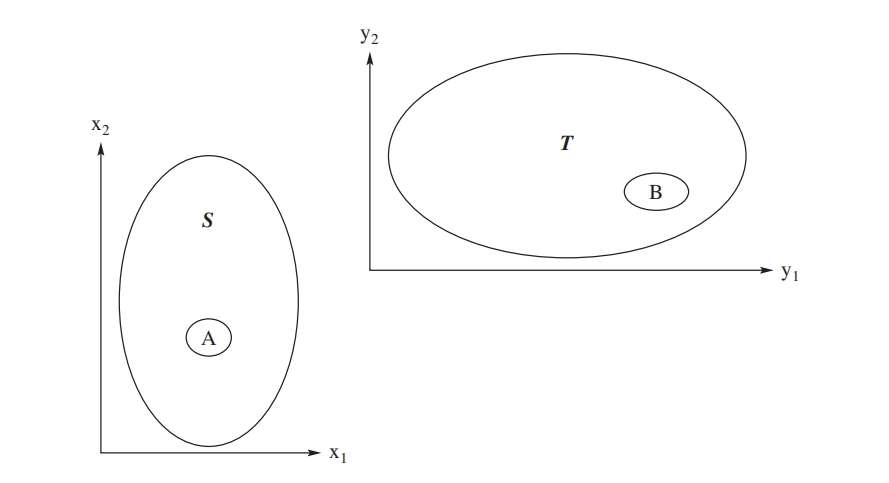
\includegraphics[width=0.6\textwidth]{figure/transformation_S_T.png}
    \caption{}
    \label{fig:transformation_S_T}
\end{figure}


\section{Conditional Distributions and Expectations}
In Section 2.1 we introduced the joint probability distribution of a pair of random
variables. We also showed how to recover the individual (marginal) distributions
for the random variables from the joint distribution. In this section, we discuss
conditional distributions, i.e., the distribution of one of the random variables when
the other has assumed a specific value.

Let the joint pmf of a discrete random vector $(X_1,X_2)$ be $p(x_1,x_2)$,
then the conditional pmf of $X_2$, given $X_1=x_1$, is
\begin{align*}
    p_{X_2|X_1}(x_2|x_1) = P(X_2=x_2|X_1=x_1)=\frac{P(X_1=x_1,X_2=x_2)}{P(X_1=x_1)}=\frac{p(x_1,x_2)}{p_{X_1}(x_1)},
\end{align*}


We now introduce a parameter $\rho$ of the joint distribution of $(X,Y)$ 
which quantifies the dependence between $X$ and $Y$ (so that $\rho=0$ when $X$ and $Y$ are independent).
We assume the existence of all expectation under discussion.

\begin{definition}{}{}
    Let $(X,Y)$ have a joint distribution. Denote the means of $X$ and $Y$
    respectively by $\mu_1$ and $\mu_2$ and their respective variances by $\sigma_1^2$ and $\sigma_2^2$.
    The covariance of $(X,Y)$ is 
    \begin{align*}
        \text{cov}(X,Y) = E[(X-\mu_1)(Y-\mu_2)].
    \end{align*}
\end{definition}

\begin{remark}
    Since the expectation operator is linear, then
    \begin{align*}
        \text{cov}(X,Y) &= E[XY-\mu_2X-\mu_1Y+\mu_1\mu_2] = E[XY] - \mu_2E[X] - \mu_1 E[Y] +\mu_1\mu_2\\
                        &= E[XY] - \mu_1\mu_2-\mu_1\mu_2+\mu_1\mu_2 = E[XY] - \mu_1\mu_2. 
    \end{align*}
\end{remark}

\begin{definition}{}{}
    If each of $\sigma_1$ and $\sigma_2$ is positive then the correlation coefficient between $X$ and $Y$ is 
    \begin{align*}
        \rho = \frac{E[(X-\mu_1)(Y-\mu_2)]}{\sigma_1\sigma_2} = \frac{\text{cov}(X,Y)}{\sigma_1\sigma_2}.
    \end{align*}
\end{definition}

\begin{remark}
    We can relate these parameters as
    \begin{align*}
        E[XY]  &=\mu_1\mu_2 +\text{cov}(X,Y)\\
            &= \mu_1\mu_2 +\rho\sigma_1\sigma_2.
    \end{align*}
\end{remark}

\begin{theorem}{}{}
    For all jointly distributed random variables $(X,Y)$ whose correlation coefficient $\rho$ exists
    (so that $\sigma_1>0$ and $\sigma_2>0$ by the definition of $\rho$), we have $-1\leqs \rho \leqs 1$.
\end{theorem}

\begin{theorem}{}{}
    If $X$ and $Y$ are independent random variables then $\text{cov}(X,Y)=0$ and hence $\rho=0$.
\end{theorem}

\begin{theorem}{}{}
    Suppose $(X,Y)$ have a joint distribution with the variances of $X$ and $Y$ finite and positive.
    Denote the means and variances of $X$ and $Y$ by $\mu_1,\mu_2$ and $\sigma_1^2,\sigma_2^2$, respectively,
    and let $\rho$ be the correlation coefficient between $X$ and $Y$. If $E[Y|X]$ is linear in $X$ then
    \begin{align*}
        E[Y|X] = \mu_2 + \rho \frac{\sigma_2}{\sigma_1}(X-\mu_1) \text{ and }\\
        E[Var(Y|X)] = \sigma_2^2(1-\rho^2).
    \end{align*}
\end{theorem}



\section{Independent Random Variables}

\section{The Correlation Coefficient}

\section{Homework}

\begin{exercise}{2.3.6}{}
    Let the joint pdf of $X$ and $Y$ be given by
    \begin{align*}
        f(x,y) = \left\{\begin{matrix}
            \frac{2}{(1+x+y)^3} & 0<x<\infty, 0<y<\infty\\
            0 & \text{elsewhere}.
           \end{matrix}\right.
    \end{align*}
    (a) Compute the marginal pdf of $X$ and the conditional pdf of $Y$, given $X=x$.\\
    (b) For a fixed $X=x$, compute $E(1+x+Y|x)$ and use the result to compute $E(Y|x)$.
\end{exercise}

\begin{solve}
    (a) By the definition of marginal probability density function:
    \begin{align*}
        f_X(x)&= \int_{-\infty}^{\infty}f(x,y)dy=\int_{0}^{\infty} \frac{2}{(1+x+y)^3} dy\stackrel{t=1+x+y}{=}\int_{1+x}^{\infty}\frac{2}{t^3}dt\\
              &= -t^{-2}|_{t=1+x}^{t=\infty} = 0-(-(1+x)^{-2})=\frac{1}{(1+x)^2}, \text{ for } 0<x<\infty.\\
        f_Y(y)&= \int_{-\infty}^{\infty}f(x,y)dx=\int_{0}^{\infty} \frac{2}{(1+x+y)^3} dx\\
              &= \frac{1}{(1+y)^2}, \text{ for } 0<y<\infty.
    \end{align*}
    Hence, $f_X(x)=\left\{\begin{matrix}
       \frac{1}{(1+x)^2} & 0<x<\infty \\
       0 & \text{elsewhere}
       \end{matrix}\right.$
    and $f_Y(y)=\left\{\begin{matrix}
        \frac{1}{(1+y)^2} & 0<y<\infty \\
        0 & \text{elsewhere}
        \end{matrix}\right.$.
    \par
    The conditional probability density function of $Y$ given $X=x$ is 
    \begin{align*}
        f_{Y|X}(y|x)=\frac{f_{X,Y}(x,y)}{f_X(x)}=\frac{\frac{2}{(1+x+y)^3}}{\frac{1}{(1+x)^2}}=\frac{2(1+x)^2}{(1+x+y)^3}, \text{ for } 0<x<\infty.
    \end{align*}
    Hence, $f_{Y|X}(y|x)=\left\{\begin{matrix}
        \frac{2(1+x)^2}{(1+x+y)^3} & 0<y<\infty \\
        0 & \text{elsewhere}.
        \end{matrix}\right.$
    \par
    (b) The conditional expectation of $g(Y)=1+X+Y$ given $X=x$ is
    \begin{align*}
        E(1+x+Y|x) &= \int_{-\infty}^{\infty} g(y) f_{Y|X}(y|x) dy\\
                   &= \int_{0}^{\infty} (1+x+y)\frac{2(1+x)^2}{(1+x+y)^2} dy\\
                   \stackrel{t=1+x+y}{=} &\int_{1+x}^{\infty} \frac{2(1+x)^2}{t^2}dt=-\frac{2(1+x)^2}{t}|_{t=1+x}^{t=\infty}=2(1+x).
    \end{align*}
    Since $E(1+x+Y|x)=1+x+E(Y|x)$, $E(Y|x)=2(1+x)-(1+x)=(1+x)$.
\end{solve}





\begin{exercise}{2.6.9}{}
    Let $X_1,X_2,X_3$ be iid with common pdf $f(x)=\exp(-x)$, $0<x<\infty$,
    zero elsewhere. Evaluste:\\
    (a) $P(X_1<X_2|X_1<2X_2)$.\\
    (b) $P(X_1<X_2<X_3|X_3<1)$.
\end{exercise}
\begin{solve}
    The joint common pdf of $X_1,X_2$ is
    \begin{align*}
        f_{X_1,X_2}(x_1,x_2)= \left\{\begin{matrix}
            e^{-(x_1+x_2)} & 0<x_1<\infty,0<x_2<\infty\\
            0 & \text{elsewhere}
            \end{matrix}\right.
    \end{align*}
    The joint common pdf of $X_1,X_2,X_3$ is 
    \begin{align*}
        f_{X_1,X_2,X_3}(x_1,x_2,x_3)= \left\{\begin{matrix}
            e^{-(x_1+x_2+x_3)} & 0<x_1<\infty,0<x_2<\infty,0<x_3<\infty \\
            0 & \text{elsewhere}
            \end{matrix}\right.
    \end{align*}
    (a) Since
    \begin{align*}
        P(X_1<X_2,X_1<2X_2)&=\int_{0}^{\infty}dx_1\int_{x_1}^{\infty}e^{-(x_1+x_2)} dx_2 = \int_{0}^{\infty}-e^{-x_1}e^{-x_2}|_{x_2=x_1}^{x_2=\infty}dx_1\\
                           &= \int_{0}^{\infty}0-(-e^{-2x_1})dx_1\\
                           &= -\frac{1}{2}e^{-2x_1}|_{x_1=0}^{x_1=\infty}\\
                           &= \frac{1}{2}
    \end{align*}
    and 
    \begin{align*}
        P(X_1<2X_2)&=\int_{0}^{\infty}dx_1\int_{\frac{x_1}{2}}^{\infty}e^{-(x_1+x_2)} dx_2 = \int_{0}^{\infty}-e^{-x_1}e^{-x_2}|_{x_2=\frac{x_1}{2}}^{x_2=\infty}dx_1\\
                           &= \int_{0}^{\infty}0-(-e^{-x_1}e^{-\frac{x_1}{2}})dx_1\\
                           &= -\frac{2}{3}e^{-\frac{3}{2}x_1}|_{x_1=0}^{x_1=\infty}\\
                           &= \frac{2}{3},
    \end{align*}
    $P(X_1<X_2|X_1<2X_2)=\frac{P(X_1<X_2,X_1<2X_2)}{P(X_1<2X_2)}=\frac{\frac{1}{2}}{\frac{2}{3}}=\frac{3}{4}$.
    \par
    (b) Since
    \begin{align*}
        P(X_1<X_2<X_3,X_3<1)&=\int_{0}^{1}\{\int_{0}^{x_3}\{\int_{0}^{x_2}e^{-(x_1+x_2+x_3)} dx_1\}dx_2\}dx_3\\
                            &=\int_{0}^{1}\{\int_{0}^{x_3}-e^{-(x_1+x_2+x_3)}|_{x_1=0}^{x_1=x_2}dx_2\}dx_3\\
                            &=\int_{0}^{1}\{\int_{0}^{x_3}-e^{-(2x_2+x_3)}+e^{-(x_2+x_3)}dx_2\}dx_3\\
                            &= \int_{0}^{1} \frac{1}{2}e^{-(2x_2+x_3)}-e^{-(x_2+x_3)}|_{x_2=0}^{x_2=x_3}dx_3\\
                            &= \int_{0}^{1} \frac{1}{2} e^{-x_3} -e^{-2x_3}+\frac{1}{2}e^{-3x_3}dx_3\\
                            &= -\frac{1}{2}e^{-x_3}+\frac{1}{2}e^{-2x_3}-\frac{1}{6}e^{-3x_3}|_{x_3=0}^{x_3=1}\\
                            &= -\frac{1}{2}e^{-1} + \frac{1}{2}e^{-2}-\frac{1}{6}e^{-3}+\frac{1}{6}
    \end{align*}
    and 
    \begin{align*}
        P(X_3<1) = \int_{0}^{1} e^{-x} dx = -e^{-x}|_{x=0}^{x=1}=-e^{-1}+1,
    \end{align*}
    $P(X_1<X_2<X_3|X_3<1)=\frac{P(X_1<X_2<X_3,X_3<1)}{P(X_3<1)}=\frac{1-3e^{-1}+3e^{-2}-e^{-3}}{6(1-e^{-1})}$.
\end{solve}



\section{Reference}
\begin{itemize}
    \item \href{https://ccrgpages.rit.edu/~whelan/courses/2013_3fa_STAT_405/notes02.pdf}{chapter 2}
    \item \href{https://faculty.etsu.edu/gardnerr/4047/notes-Hogg-McKean-Craig/Hogg-McKean-Craig-2-1.pdf}{2.1}
    \item \href{https://faculty.etsu.edu/gardnerr/4047/notes-Hogg-McKean-Craig/Hogg-McKean-Craig-2-3.pdf}{2.3}
    \item \href{https://tomoki-okuno.com/files/math/Ch2_sol.pdf}{ch2 solution}
\end{itemize}